\documentclass[10pt, a4paper]{article}
\usepackage[T1]{fontenc}
\usepackage[utf8]{inputenc}
%\usepackage[swedish]{babel}
\usepackage{ifpdf}
\usepackage[parfill]{parskip}
\usepackage{graphicx}
\usepackage{fancyvrb}   % For source code listing.
\fvset{tabsize=4}       % Tabstop is 4 spaces.
\fvset{fontsize=\small} % Small fonts for source code.

\title{EDA031 Project - News System}
%\date{}
\author{
	\begin{tabular}{l l}
		Erik Westrup & \texttt{<ada09ewe@student.lu.se>}\\
		Joachim Nelson & \texttt{<ada08jne@student.lu.se>} \\ % TODO rätt mail?
		Oscar Olsson & \texttt{<ada09ool@student.lu.se>}
	\end{tabular}
}

\begin{document}

\begin{titlepage}
\maketitle
\thispagestyle{empty}	% No page number on title page.
\end{titlepage}
%\setcounter{page}{2}

\section{EDA031 Project - News System}
The purpose of the project was to develop a simple news system consisting of a client and server model. The objects of interest for the user is news articles. An article is have a title, is written by an author and contains text content. Articles are created by users using a client and are posted to different news groups. Each article belongs to one news group and are stored in a database at the server side. In total, the allowed operations from the users are listing news groups, listing articles in a specified news group, reading an article, creating articles, deleting articles and news groups.

The server was required to have a memory database and a persistent file database. The file database was implemented with one directory on disk for each news group and the articles as text files in these directories. The communication between the server and client uses a specified protocol in the application layer on top of TCP/IP. The server needed not be be multi-threaded but should sequentially be able to handle multiple clients.

\section{Detailed description of design and UML}
From the beginning we realized that the server and client will share much of the functionality related to network communication and data representation. We decided to make a net package containing classes dealing with communication. The package should of course be independent of client and server. Early on we also discussed if the information (result to queries)  at the server side could be reused at the client side. Later in the project this led to a database package DB containing both queries and the accompanying results that can be used on either side of the communication. However only one side needs to know how to send queries and the other how to receive and the reverse situation for the results. These parts was therefore split in and put at the server and client packages.

To meet the requirement of two databases we decided it would be best to make a database interface and to implemented that in a file and memory version. Our initial design is show in figure \ref{init+design}.

\begin{figure}[hbt]
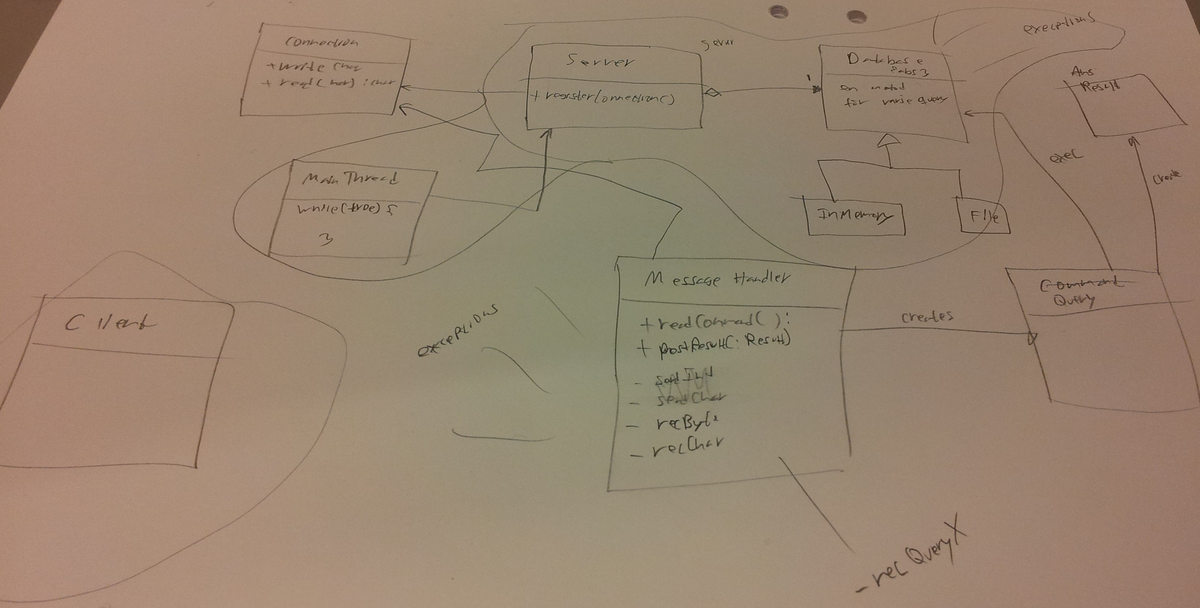
\includegraphics[scale=0.4]{img/uml_blueprint.png}
\label{init+design}
\caption{Initial design after our first project meeting.}
\end{figure}
\begin{figure}[hbt]


In the final version of the system we had not deviated too much from the original design. The main difference is the previously mentioned separation of receiving and sending queries and results. A UML diagram of the final design can be seen in figure \ref{UML}.

\begin{center}
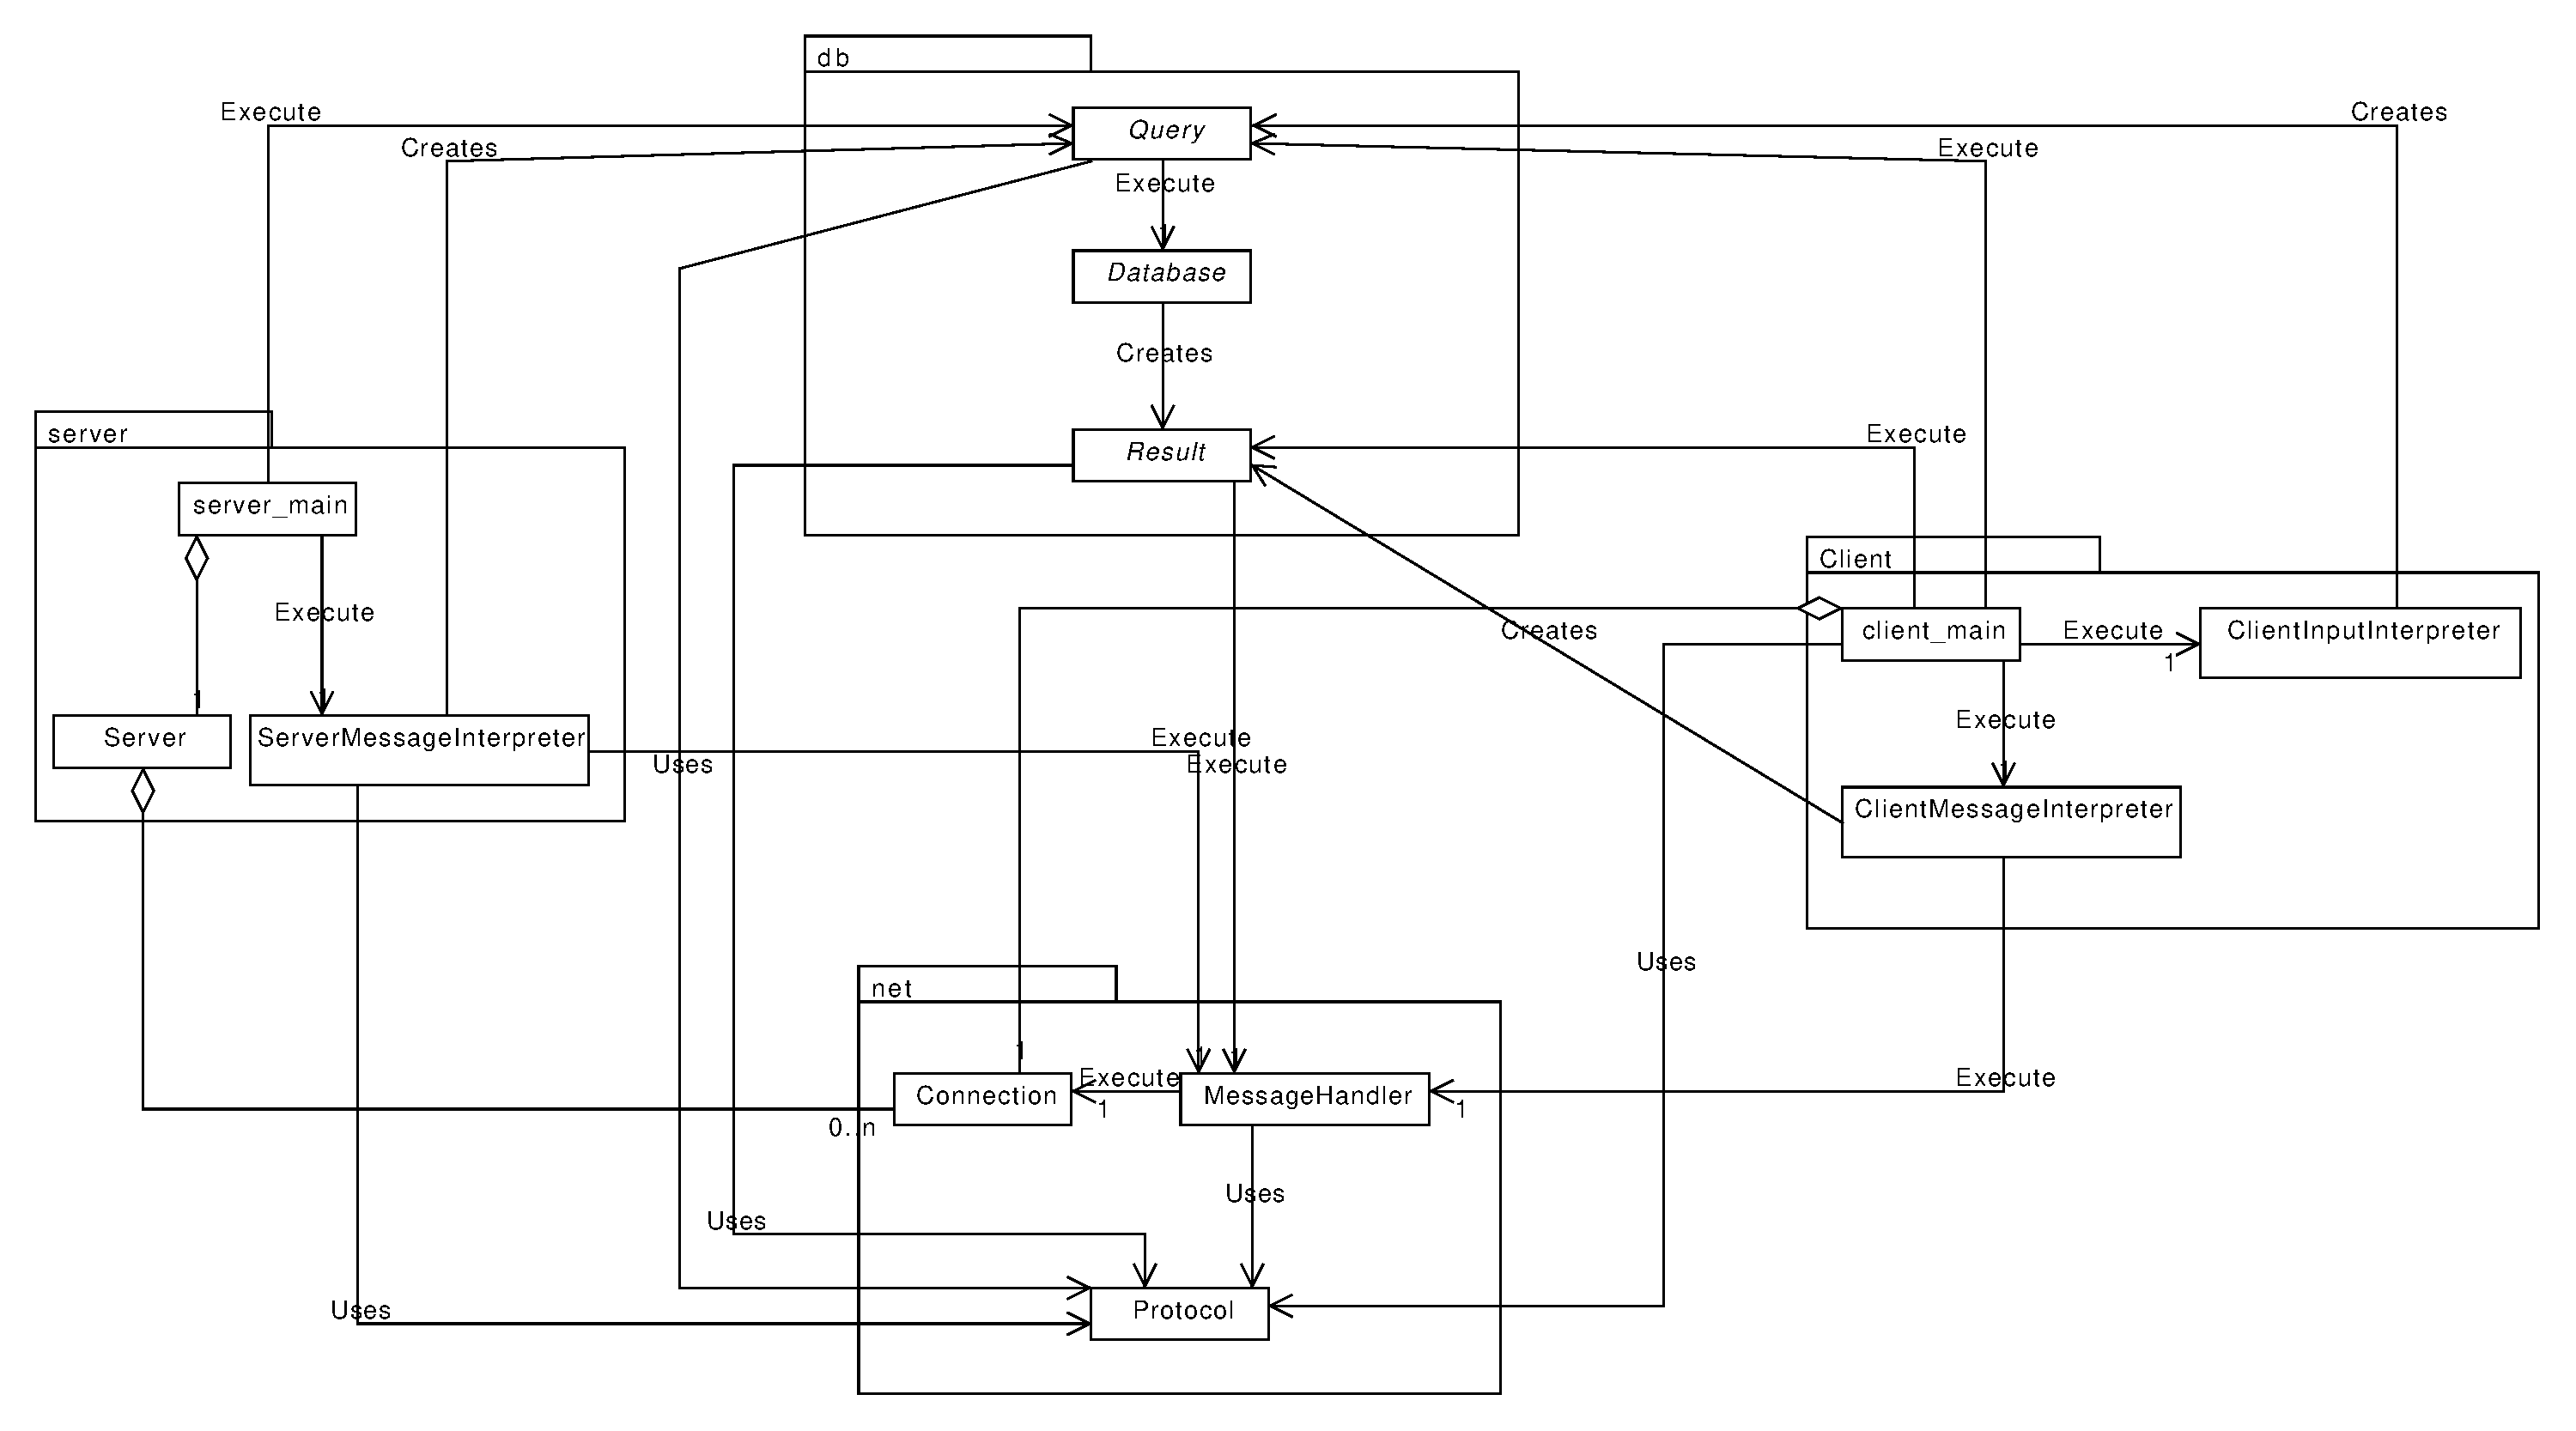
\includegraphics[scale=0.3]{img/uml.pdf}
\end{center}
\label{UML}
\caption{An UML diagram describing the project.}
\end{figure}

\subsection{Net}
Most of the functions needed for using UNIX sockets were given to use from the beginning. We did not need to change them, only put them in this package. The reason for this is probably that the projects goal was to practice C++ and STL, not UNIX programming.

\subsection{DB}
\subsection{Client}
\subsection{Server}
The server package consists most importantly of the main function found in \emph{server/server\_main}. It first register it self as listener at a port in the operating system. It then wait for events of two types, new connections, disconnections and command requests from existing connections. In the first case the connection is stored, in the second deregistered. In the third case when a request is made the class \emph{ServerMessageInterpreter} is invoked. It knows how to receive queries and used the protocol \emph{net/protocol.h} and the \emph{MessagHandler} to construct a \emph{Query} object. The query is then executed against the database interface which returns a \emph{Result} object. That result knows it data and thus sends it self on the network using a \emph{MessageHandler} for data conversion.

\subsection{Communication, flow-chart}

\subsection{Conclusion}


We also took the chance of trying the front end clang to LLVM after an inspiring guest lecture by Hans Wennborg in the course. We found that it was easier to work with since it produced cleaner and colored output. It also gave useful suggestions to causes and solution to the problems.

\subsubsection{Implemented requirements}

\subsubsection{Problems}
This was our first project developed with C++ and could potentially caused us many problems. However it went surprisingly well and there were relative few problems. We had previous experience from the tools used like GCC, GNU Make, valgrind etc. One obstacle though was to make good Makefile. We wanted all compiled files to be put in a build directory and thus not pollute the source tree. That is fairly simple, just change the path with pattern substitution. But we also wanted to have automatic generation of dependencies so we don't have to update the Makefile each time we include something new. Thus we want a Makefile for each .cc-file. Examples on how to do that have been used in the course and take from the GNU Make manual section 4.4 \cite{makeman}. Also we wanted the structure on disk to reflect the programs logical division in namespaces.

However the combination separate output directory, automatic prerequisites generation and structural directories proved to be a daunting task. After days of hacking, manual consultation and testing it was found that the automatic compilation targets for .cc-files to .o-files that the solution from the manpages was never invoked when the target destination is not the same as the prerequisite. This had to be solved with some really ugly hacks but we got it working. At least we are now eager to start using tools from the GNU build system or CMake to escape the task of writing Makefiles.


\subsubsection{Missing features}
We believe that we have implemented all features outlined in the specification.

\subsubsection{Suggestions}




\emph{\cite{dummy+ref}} 
\newpage
\bibliographystyle{plain}
\bibliography{references}
\end{document}

%\begin{figure}[hbt]
%\begin{center}
%\includegraphics[scale=0.4]{img/pic1.png}
%\end{center}
%\label{LABEL}
%\caption{DESCRIPTION text.}
%\end{figure}
%\clearpage

%\VerbatimInput{src/prog1.c}
